\documentclass[a4paper,twocolumn]{article}
\usepackage[a4paper,margin=2cm]{geometry} % Seitenränder anpassen
\usepackage{graphicx} % Für Grafiken
\usepackage{amsmath, amssymb} % Für mathematische Formeln
\usepackage{hyperref} % Für Hyperlinks
\usepackage{caption} % Für Bildunterschriften
\usepackage[printonlyused]{acronym}
\usepackage{pgffor} % Paket für die foreach-Schleife
\usepackage{shellesc} % Für das Ausführen von Shell-Befehlen (mit pdflatex -shell-escape)
\usepackage{todonotes}

% Abstand zwischen den Spalten erhöhen
\setlength{\columnsep}{1cm} 

\title{Augmented Reality with Aruco Markers}
\author{
    Hochschule Ravensburg-Weingarten \\[1em] % Hochschule zentriert
    \begin{minipage}[t]{0.45\textwidth} % Linke Spalte
        \centering
        Jonas Alber \\ % Name
        15444427\\
        \texttt{jonas.alber@hs-weingarten.de} % E-Mail
    \end{minipage}
    \hfill
    \begin{minipage}[t]{0.45\textwidth} % Rechte Spalte
        \centering
        Tim Schweitzer \\  29844429 \\ % Name
        \texttt{tim.schweitzer@hs-weingarten.de} % E-Mail
    \end{minipage}
}
\date{\today}

\begin{document}

\maketitle

\section*{Disclaimer}

Der Inhalt dieses Dokuments wurde von den oben genannten Autoren erstellt. Zur Verbesserung der Lesbarkeit wurde ChatGPT von OpenAI genutzt. Sämtliche Inhalte wurden jedoch von den Autoren geprüft und gegebenenfalls angepasst.


\section*{Abkürzungsverzeichnis}
\begin{acronym}[RWU]
    \acro{RWU}{Hochschule Ravensburg Weingarten}
    \acro{AI}{Artificial Intelligence}
    \acro{IoT}{Internet of Things}
\end{acronym}

\begin{abstract}

\end{abstract}

\section{Einleitung}

\subsection{Aufgabenstellung}
Diese Arbeit wurde im Rahmen des Fachs Computer Vision an der \ac{RWU} als Projektaufgabe erstellt. Ziel des Projekts ist es, mithilfe der Bibliothek OpenCV Bilder so zu modifizieren, dass ein Poster derart in das Bild integriert wird, dass für den Betrachter der Eindruck entsteht, das Poster befinde sich tatsächlich im Raum.
\\
Diese Bildaugmentierung wird auf einen vorgegebenen Datensatz angewendet, wobei die erzielten Ergebnisse anschließend auf selbst erstellte Bilder übertragen werden sollen.

\subsection{Marker}
\todo{Fehlende Quelle!}
Eine zentrale Herausforderung in allen Disziplinen der Informatik, die mit Bilddaten arbeiten, besteht in der Interpretation von Räumlichkeiten auf Basis einzelner Perspektiven. Ein vielversprechender Ansatz zur Erkennung von Orientierung und Ausrichtung ist die Nutzung von Markern.
\\
Im Rahmen dieser Arbeit wird der ArUco-Marker eingesetzt. Dabei handelt es sich um speziell entwickelte Marker, die aus einem quadratischen schwarz-weißen Muster bestehen und eine eindeutige Identifizierung sowie die Berechnung von Position und Ausrichtung im Raum ermöglichen. \cite{aruco1}

\section{Image Transformation Process}
The image transformation process begins by loading the input image \ref{fig:example-base}, which contains ArUco markers, as well as the poster (Figure \ref{fig:img-poster}) image. 
\begin{figure}[h!]
    \centering
    \includegraphics[width=0.9\columnwidth]{img/img_base_113340.jpg} % Beispielbild
    \caption{Fernaufame des Arucumarkers aus dem Vorgegbeenen Datensatz.\cite{stefan-elser}}
    \label{fig:example-base}
\end{figure}
\\
The script then scales and adjusts the poster dimensions to fit within the area defined by the detected ArUco marker, ensuring the poster aligns properly with the marker's size and orientation. To achieve this, the script calculates the corners of the scaled poster and determines their correct positions relative to the marker's location. 
\\
Next, the ArUco markers are detected within the image using OpenCV's aruco.detectMarkers function, which identifies the marker's corners. A perspective transformation matrix is calculated based on the positions of the poster corners and the detected marker corners. This matrix is then used to warp the poster image so that it aligns precisely with the detected marker area.
\begin{figure}[h!]
    \centering
    \includegraphics[width=0.9\columnwidth]{img/detectedMarker_113340.jpg} % Beispielbild
    \caption{Detected Marker Image.\cite{stefan-elser}}
    \label{fig:detected-marker}
\end{figure}
\\
To integrate the transformed poster into the original image, a mask is created, which isolates the transformed poster region. The mask is then inverted so that only the region outside the poster area is kept, ensuring that the poster seamlessly blends with the background. Finally, the mask is applied to the image, and the transformed poster is combined with the original image using bitwise operations, resulting in the final image with the poster placed correctly within the marker-defined region.

\section{Evaluation and Validation}

Once the image transformation is complete, the script proceeds to evaluate the alignment of the poster placement.
\begin{figure}[h!]
    \centering
    \includegraphics[width=0.9\columnwidth]{img/img_result_113340.jpg} % Beispielbild
    \caption{Fernaufame des Arucumarkers aus dem Vorgegbeenen Datensatz mit Poster.}
    \label{fig:example-result}
\end{figure}
 \\
 The first step in the evaluation is detecting the edges of the image using the Canny edge detection method. This process highlights the boundaries of the poster and the surrounding areas, providing a clear view of the poster's edges.
Following edge detection, the script employs the Hough Line Transform to extract the prominent lines from the edge-detected image. This method identifies and highlights the linear features within the image, including the edges of the poster. By comparing the detected lines with the expected positions of the poster's edges, the script can assess whether the poster has been placed accurately.
\\
Finally, the evaluation results are visualized by overlaying the detected lines and edges on the original image. This allows for easy manual inspection of the poster’s placement, providing immediate feedback on the transformation’s accuracy. The combination of edge detection and line extraction ensures that any misalignment or distortion in the poster placement is clearly visible for quality assurance.
\\
Bei der Analyse weiterer Bilder zeigt sich jedoch, dass die Erkennung des Aruco-Markers nicht in jeder Perspektive zuverlässig funktioniert. Ein Beispiel hierfür ist in Abbildung \ref{fig:bad-example-result} zu sehen. Beim Vergleich der horizontalen Fluchtpunktlinien des Posters(Grün) mit der Metallstange(Rot) wird sichtbar, dass die Fluchtpunktlinien mit zunehmender Entfernung immer weiter von der Stange abweichen und schließlich abweichen.
Abgesehen vom Fluchtpunkt sind die Poster in der Platzierung und dem Aspekt ratio konsistent und erlauben ein Stabiles einfügen der Poster.
\begin{figure}[h!]
    \centering
    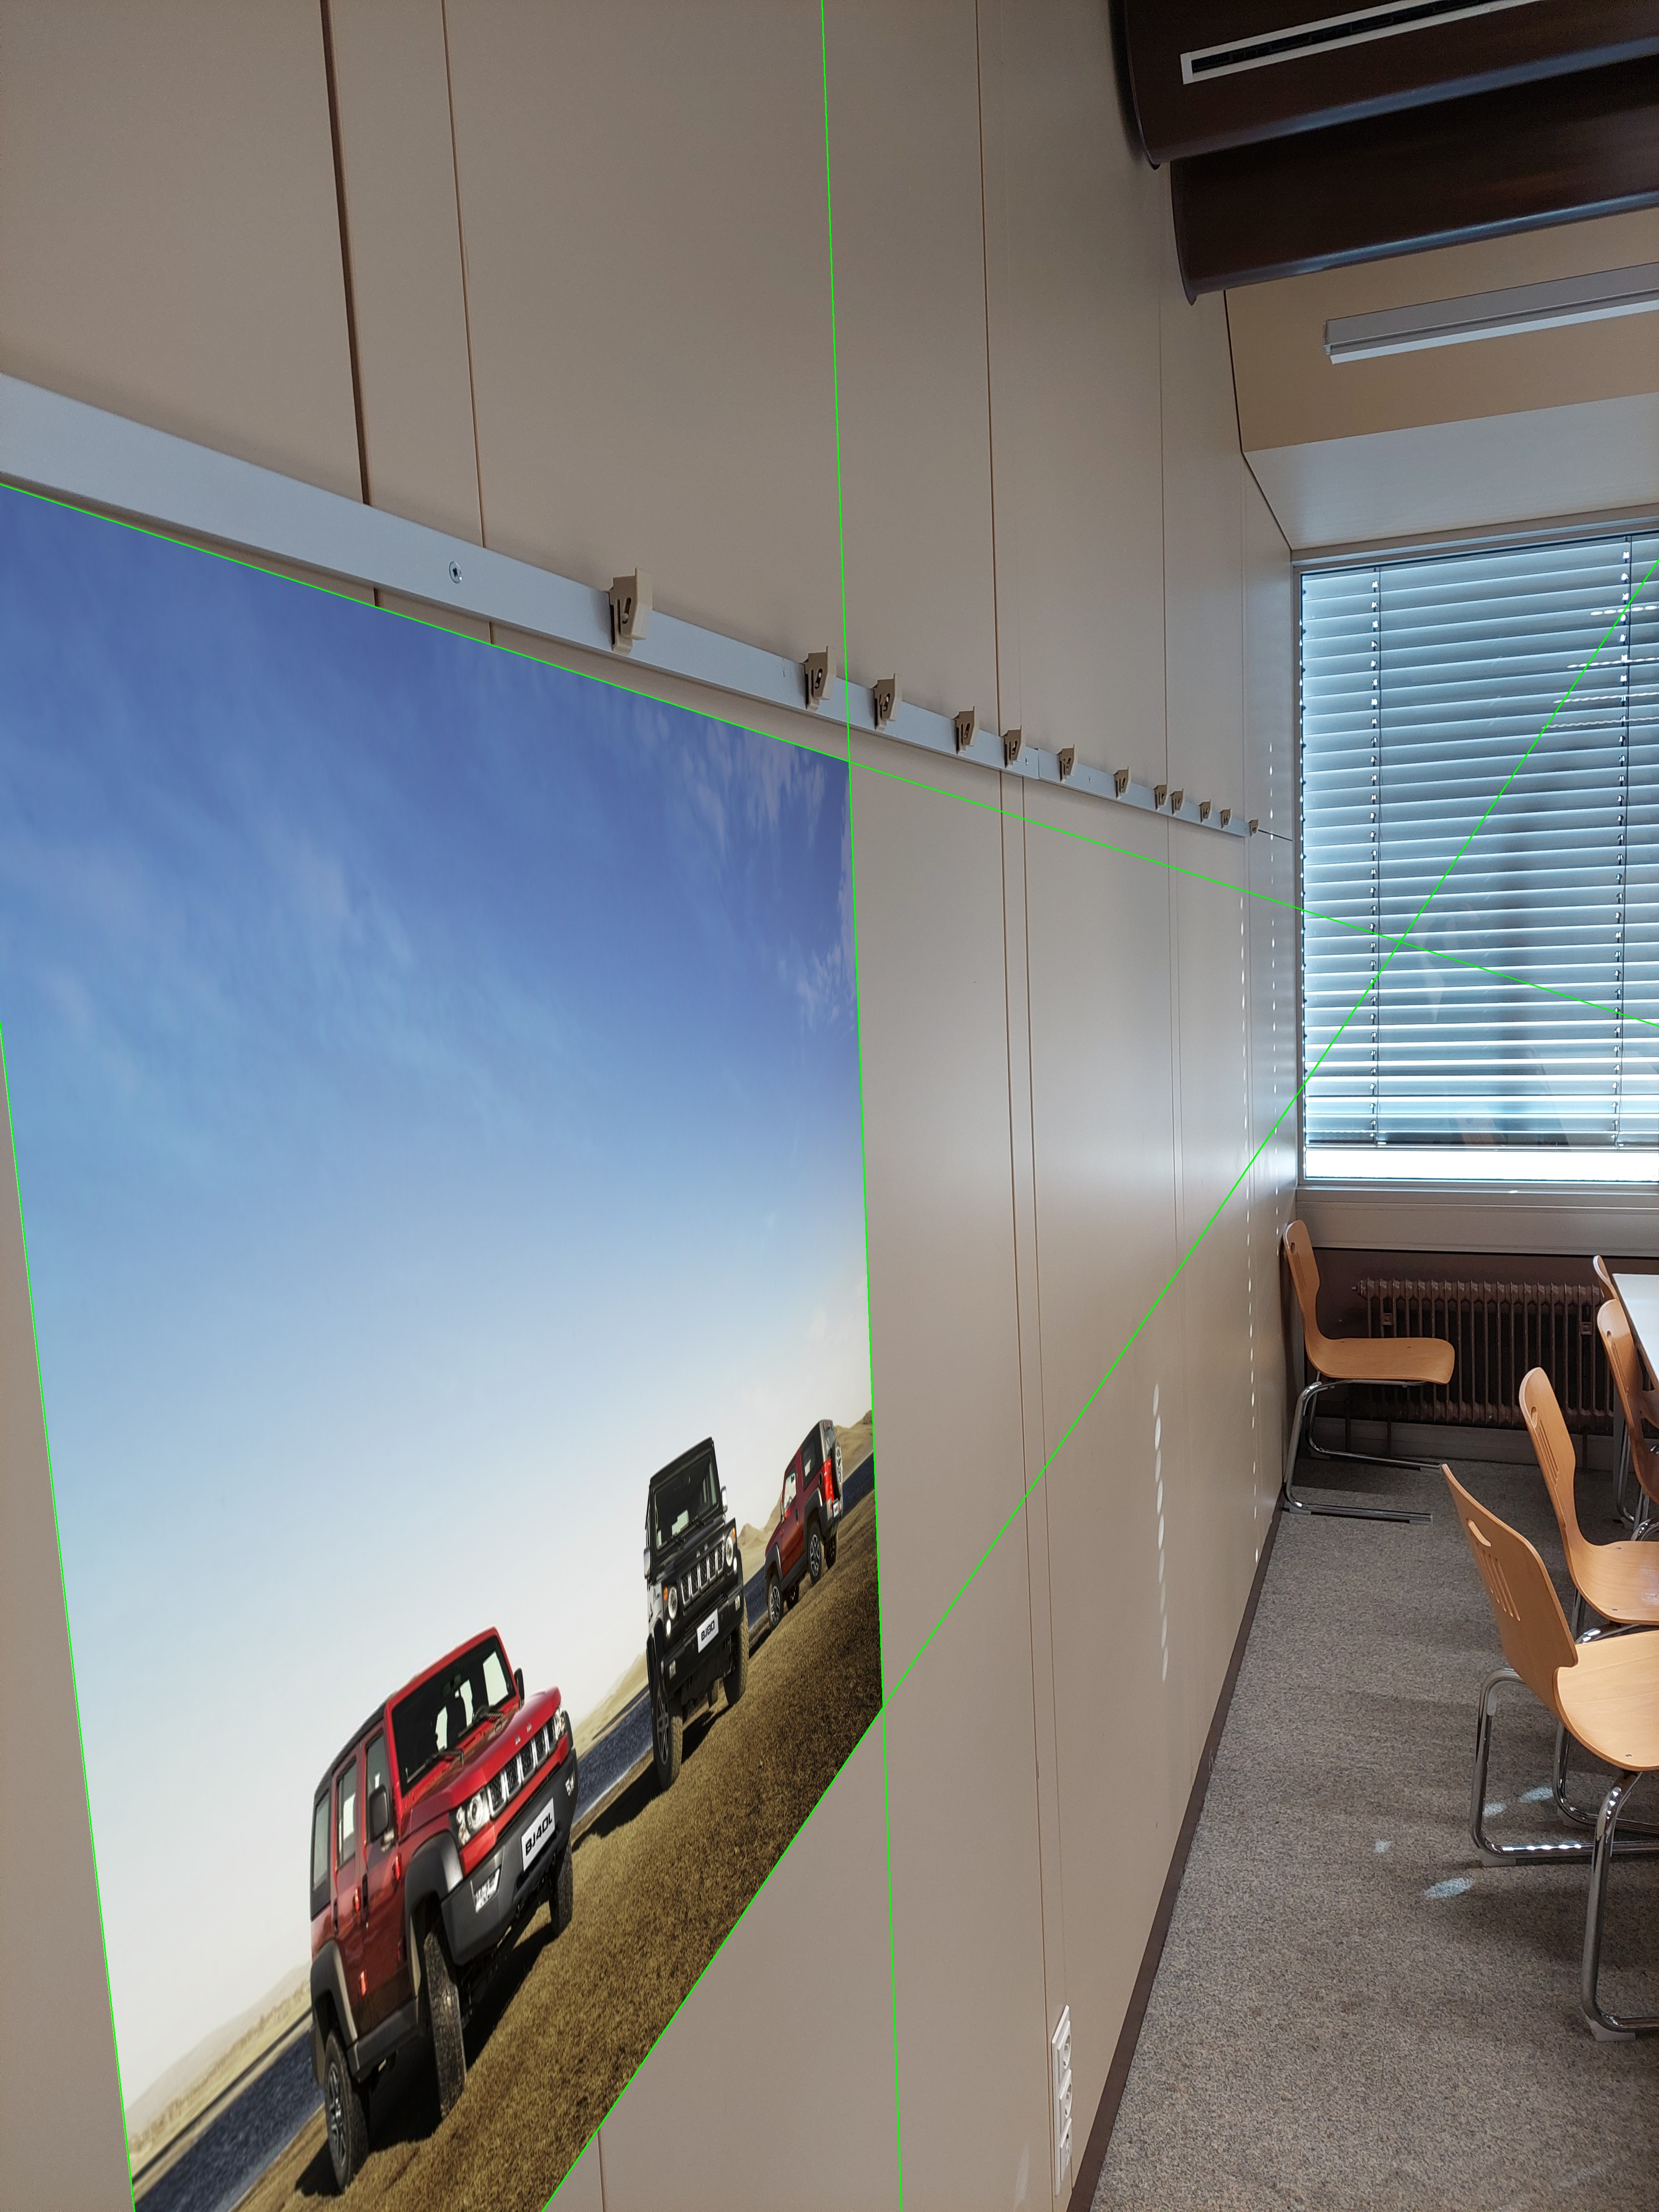
\includegraphics[width=0.9\columnwidth]{img/img_result_bad_113437.jpg} % Beispielbild
    \caption{Beispiel für eine Perspektive bei welcher der Fluchtpunkt schlecht erkannt wurde.}
    \label{fig:bad-example-result}
\end{figure}

\section{Fazit und Ausblick}

Im Rahmen dieses Projekts wurde eine Software zur Platzierung von Postern in einem Bild entwickelt. Dafür wurden hauptsächlich der Aruco-Marker und die Bibliothek OpenCV verwendet.
\\
Die Ergebnisse der Posterplatzierung sind grundsätzlich solide und positionieren das Poster in der richtigen Größe im Raum. Die Abweichung zwischen der berechneten und der tatsächlichen Verzerrung ist in den analysierten Bildern so geringfügig, dass die Fehler nicht störend wirken. Fehler sind sehr viel stärker, wenn der Arcuo Marker eine geringere Auflösung hat und deswegen die Ecken nicht genau erkannt werden.
\\
Eine Verbesserung der Marker Erkennung war im Umfang dieser Arbeit nicht möglich und könnte im Rahmen einer umfangreicheren wissenschaftlichen Untersuchung weiter optimiert werden.

%\begin{thebibliography}{99}
%\bibitem{ref1} Autor, Titel, Quelle, Jahr.
%\bibitem{ref2} Autor, Titel, Quelle, Jahr.
%\end{thebibliography}

%\end{document}
\begin{thebibliography}{9}

    \bibitem{aruco1}
    S. Garrido-Jurado, R. Muñoz-Salinas, F. J. Madrid-Cuevas, M. J. Marín-Jiménez. 
    \textit{Automatic generation and detection of highly reliable fiducial markers under occlusion}. 
    Pattern Recognition, vol. 11, no. 6, 2021.
    
    \bibitem{stackoverflow}
    \textit{Extract vanishing point from lines with OpenCV}, 
    StackOverflow user Ilke444. Available: \url{https://stackoverflow.com/questions/57535865/extract-vanishing-point-from-lines-with-open-cv}. 
    Accessed: Nov. 28, 2024.

    \bibitem{opencv}
    OpenCV.org, 
    \textit{Tutorial: ArUco detection}, 
    Available: \url{https://docs.opencv.org/4.x/d5/dae/tutorial_aruco_detection.html}. 
    Accessed: Nov. 28, 2024.

    \bibitem{tim-schweitzer}
    Tim Schweitzer \textit{Own example Images with Aruco Marker}, 2024.

    \bibitem{stefan-elser}
    Stefan Elser \textit{Image provided by Stefan Elser for this Project}, 2024.

    \bibitem{v_speed}
    v\_speed. \textit{Poster used in Images}, 2022. Available under Pixabay-Contentlicenz license: \url{https://pixabay.com/de/photos/beijing-automotive-bj40-suv-bj80-2486704/}. Accessed: November 3, 2024, 18:01.

\end{thebibliography}

\todo{Hinzufügen der anderen Bilder}

\appendix
\section*{Anhang A: Additional Images}

\begin{figure}[h!]
    \centering
    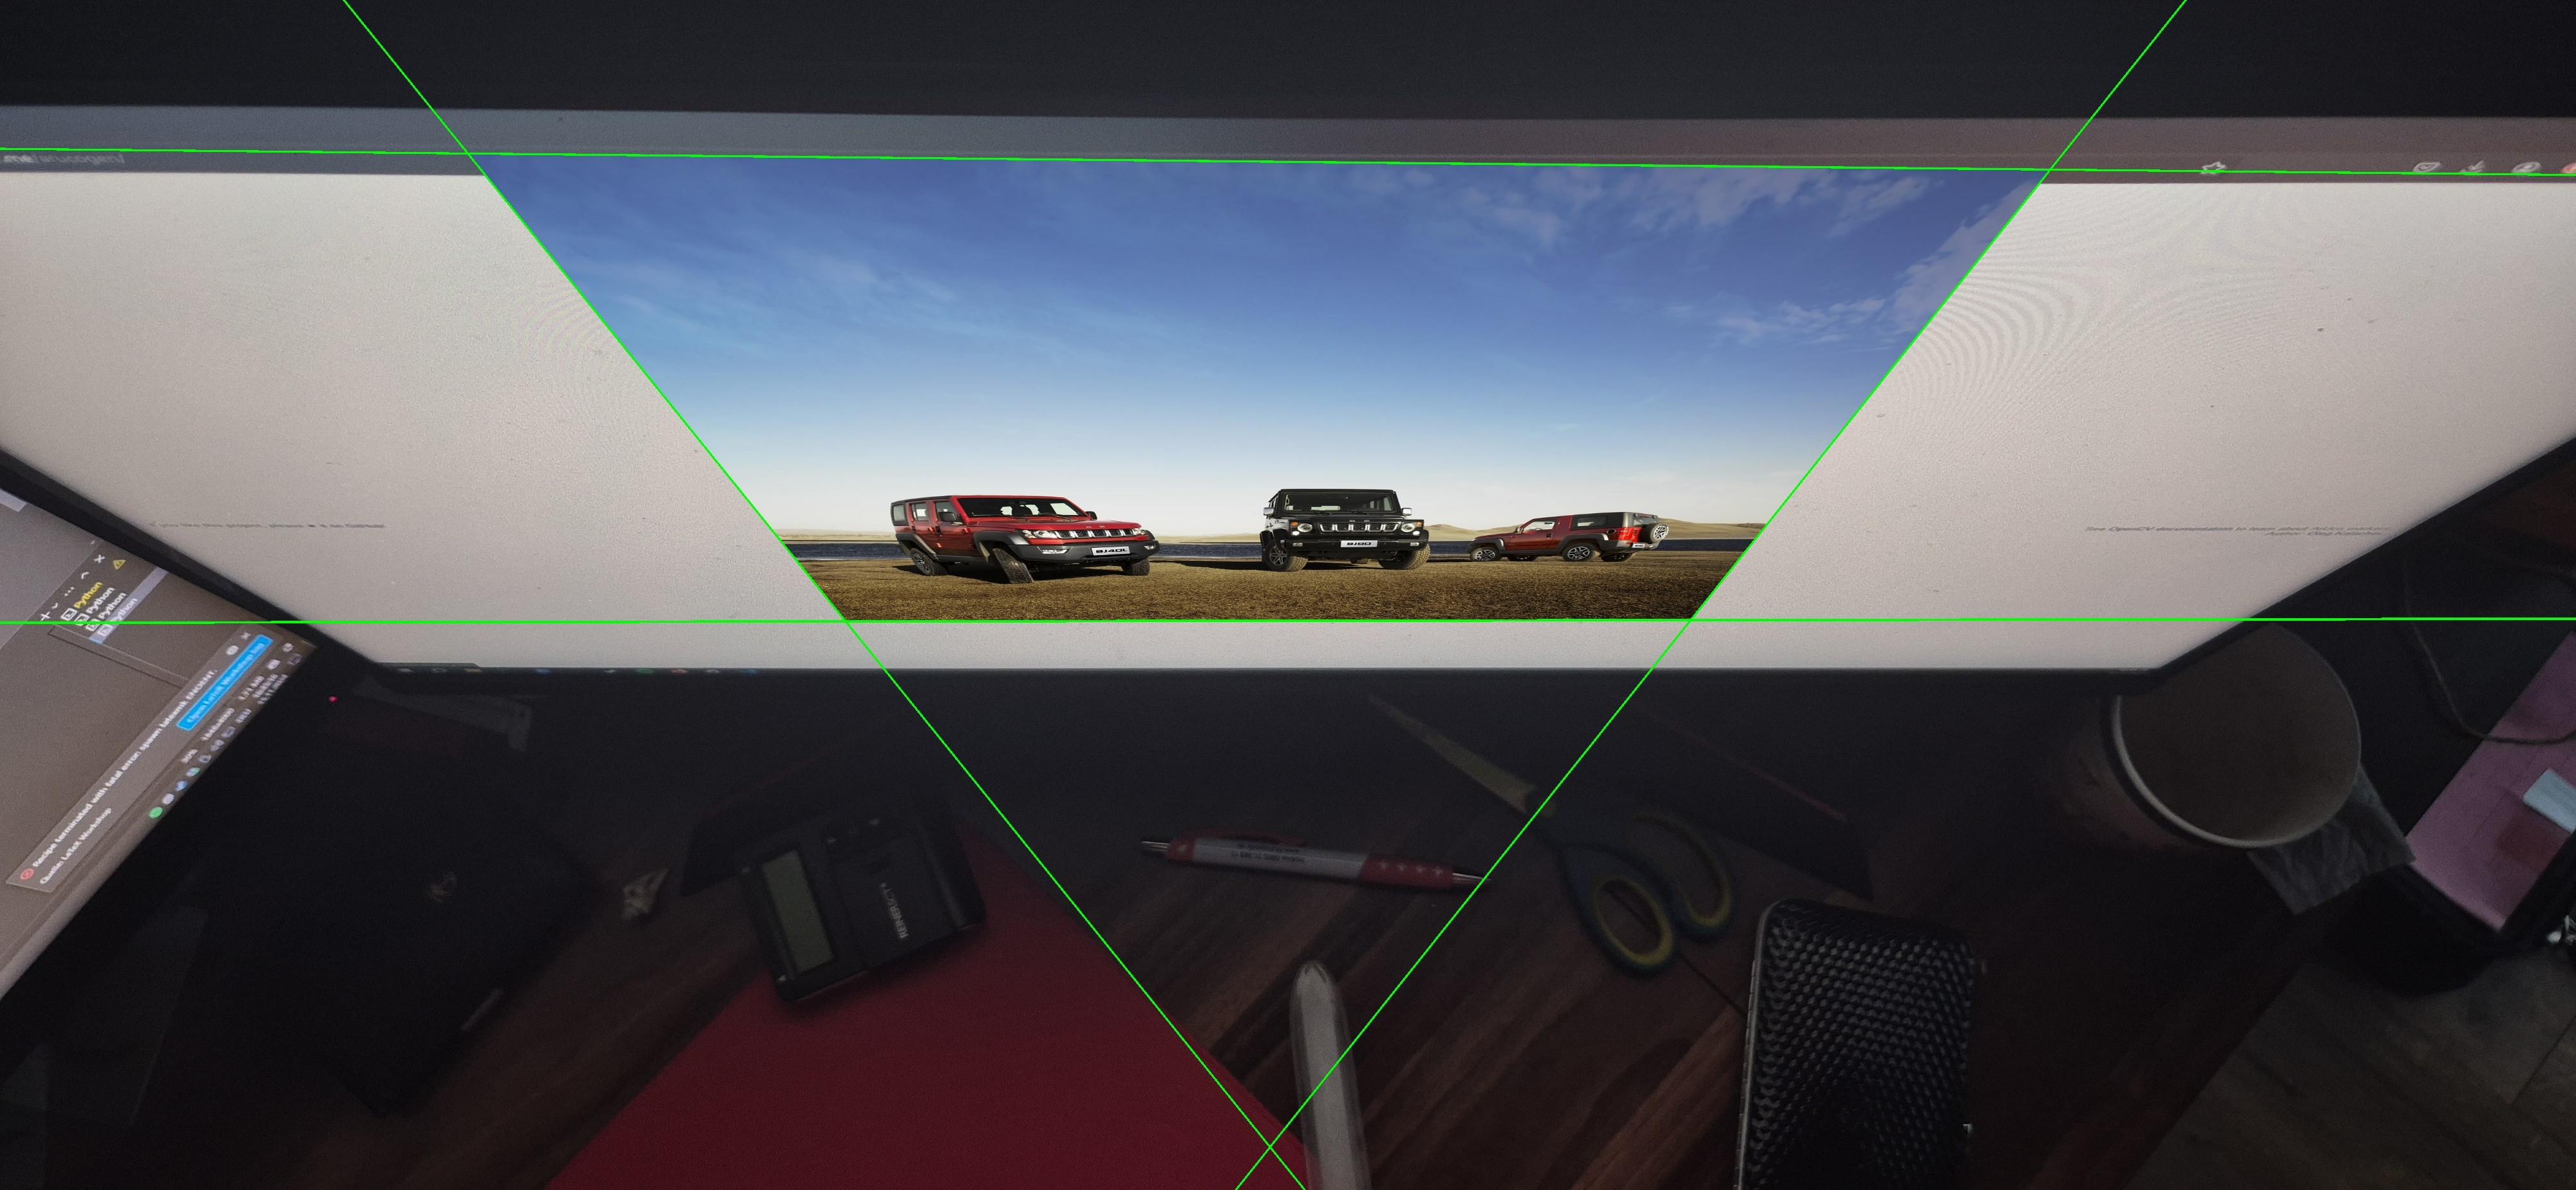
\includegraphics[width=0.9\columnwidth]{img_alt/aruco_from_screen.jpg}
    \caption{Aruco Marker on Screen \cite{tim-schweitzer}}
    \label{fig:example-appendix}
\end{figure}

\section*{Anhang B: Used Poster}

\begin{figure}[h!]
    \centering
    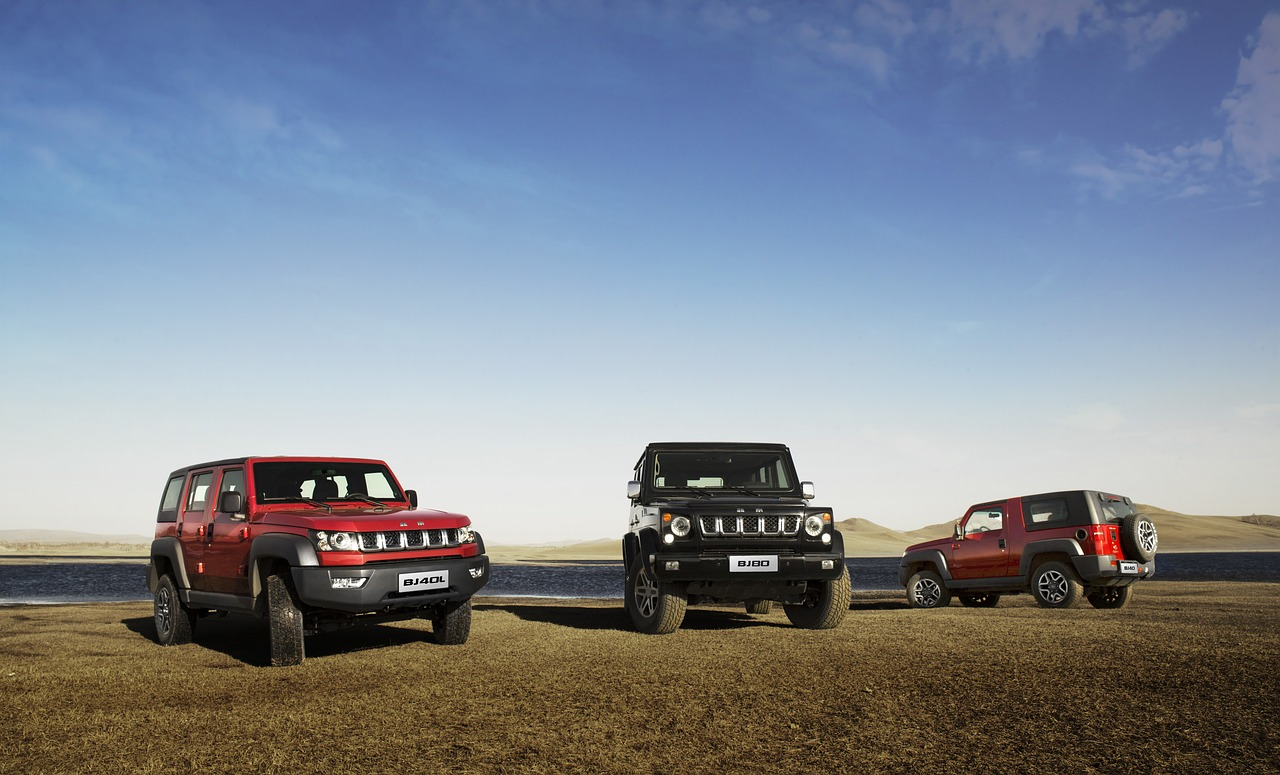
\includegraphics[width=0.9\columnwidth]{img_alt/poster.jpg}
    \caption{Poster used for Image Augmentation\cite{v_speed}}
    \label{fig:img-poster}
\end{figure}

\end{document}